\documentclass[Review, sageh, times, doublespace]{sagej} 

\usepackage{amsmath, amsfonts, array, float, graphicx, moreverb, natbib, subcaption, url, xcolor}

\usepackage[colorlinks, allcolors=blue]{hyperref}

\newcommand{\revision}[1]{{\color{orange} #1}}

\begin{document}

\runninghead{\revision{Models in the War Room}}

\title{\revision{Models in the War Room: Translating random forest predictions into player comps}}

%\author{Elisabeth Millington\affilnum{1} and Scott Powers\affilnum{2}}
%
%\affiliation{\affilnum{1}Department of Kinesiology, Rice University\\
%\affilnum{2}Department of Sport Management, Rice University}
%
%\corrauth{Scott Powers, 6100 Main St, Houston, TX, 77005}
%
%\email{scott.powers@rice.edu}

\begin{abstract}
  \revision{
    Interpretability is important for the adoption of complex predictive models, particularly in the ``war rooms'' where sports executives discuss high-stakes decisions while balancing model predictions with qualitative scouting. Especially in the context of player entry drafts, scouts often explain their assessments of prospects by identifying historical comparable prospects, or ``comps''. \citet{lin_random_2006} showed random forests are interpretable as adaptive nearest neighbors and that their predictions are recoverable as weighted averages of training outcomes. In this paper, we draw a line from this decomposition of random forest predictions to the concept of player comps, and we extract similarity scores quantifying the weight of each comp in the prediction for each prospect. This case-based approach to interpretability translates random forest predictions into the language of traditional scouting, presenting an alternative to popular feature-based approaches like SHAP values. We illustrate this approach with an application to a two-stage random forest model for predicting the professional career outcomes of collegiate quarterback prospects in American football. We provide the R package treecomp to help researchers and practitioners to extract similarity scores from their own random forest models.
  }
\end{abstract}

\keywords{American football, draft projections, ensemble methods, interpretable machine learning, scouting, sports analytics, tree-based predictions}

\maketitle

\section{Introduction}

\revision{
  In recent years, professional sports teams have leaned heavily on machine learning algorithms to support decision-making because of their potential to model complex relationships with strong predictive performance. The drawback of machine learning-based predictions is that their ``black box'' nature makes them difficult to trust blindly in high-stakes environments such as player entry drafts, in which multi-million dollar contracts and multi-year strategies hinge on individual decisions. To effectively integrate data-driven models into their decision-making, sports executives need to understand the reasoning behind the predictions so they can reconcile disagreements between models and other, often non-quantifiable, sources of information.

  Professional sports front offices already have a deeply entrenched framework for explaining forecasts of player careers: case-based reasoning using historical comparable prospects, known colloquially as ``comps'' \citep{sikkema_2025_2025}. Traditional scouting reports often identify comps whose profiles were similar to the player under evaluation, reasoning that their career outcomes portend the player's future. When a scout argues that a prospect reminds them of a successful or failed prospect from a decade earlier, they are effectively implementing a human approximation of the $k$-nearest neighbors ($k$-NN) algorithm, with $k = 1$.

  The case-based approach to interpreting predictions extends to the random forest algorithm \citep{breiman_random_2001}, which is widely favored in sports analytics for its strong predictive performance. \citet{lin_random_2006} showed that a random forest is interpretable as an adaptive $k$-NN algorithm, in which the nearness of neighbors is defined adaptively to optimize predictive performance. Instead of giving all features equal weight, the random forest learns the most important features for defining nearness to yield the best predictions. This theoretical link allows the predictions of a random forest to be recovered as a similarity-weighted average of the response values in the training data, resulting in a case-based explanation of the predictions. This is an alternative to feature-based approaches such as Shapley Additive Explanations (SHAP, \citealp{lundberg_unified_2017}), which can tell executives how features contributed to predictions but not how historical player outcomes contributed to predictions.

  The primary contribution of the present work is that we translate the predictions of a random forest model into the framework of traditional scouting. Our objective is to achieve case-based interpretability for high-performing tree ensembles, generating data-driven comps without sacrificing predictive performance. We extract similarity scores from the random forest architecture to decompose its predictions as transparent weighted averages of historical outcomes. We provide an open-source implementation in the R package treecomp, allowing practitioners and researchers to easily extract similarity scores from their own random forests fitted using randomForest \citep{breiman_randomforest_2024} and ranger \citep{wright_ranger_2017}. We illustrate the package on an application of predicting professional career outcomes using collegiate career statistics for quarterback prospects in the National Football League (NFL) Draft.
}

\subsection{Related Work}

\revision{
  Recent interpretable machine learning applications in sports analytics rely on feature-based reasoning like \textit{post hoc} SHAP values \citep{lundberg_unified_2017} to interpret complex ensemble predictions \citep{janssens_predicting_2023, ouyang_integration_2024}. Abstracting players as features does not meet the needs of sports decision-making scenarios such as player entry drafts because they cannot reveal how historical player outcomes map to new predictions. Case-based reasoning using comps aligns with the framework already entrenched in traditional scouting discussions \citep{jones_nfl_2025,sikkema_2025_2025,trapasso_nfl_2025}. While past work has used case-based reasoning to interpret random forest predictions \citep{plumb_model_2018,mazumdar_random_2021}, the present work is the first to translate the inner workings of random forests into the practical language of scouting comps.
  
  Data-driven models for player entry drafts historically force a compromise between accuracy and interpretability. Early work relied on transparent generalized linear models \citep{robbins_national_2010, wolfson_quarterback_2011, mulholland_predicting_2014, craig_predicting_2021}, failing to capture complex relationships between features and outcomes. More recent work captures these dynamics using machine learning techniques, such as principal components analysis \citep{berger_jumping_2021}, large language models \citep{luo_improving_2024}, or random forests \citep{enaganti_optimizing_2025}, at the expense of interpretability. Our approach breaks this historical compromise, preserving the predictive performance of random forests while providing case-based explanations of predictions to support high-stakes decision-making. Furthermore, unlike existing case-based sports projection systems that remain proprietary \citep{wyers_reintroducing_2012}, we provide an open-source implementation via the R package treecomp.
}

\section{Methods}
\label{sec:methods}

\revision{
  \citet{lin_random_2006} revealed the link between random forests and $k$-NN. The random forest prediction is the average of predictions of many decision trees, and each decision tree prediction is simply an average of observed outcomes in a leaf node. Therefore, the random forest prediction is a weighted average of observed outcomes, weighted by how frequently each observation occurs in the same leaf node as the observation being predicted.

  Whereas $k$-NN relies on a rigid definition of the nearness between points based on Euclidean distance, giving equal weight to all features, a random forest creates an adaptive definition of nearness to suit its prediction task. Each decision tree recursively partitions the feature space into irregular hyperrectangles (leaf nodes) determined by splits which maximize prediction performance. High-signal features (and interactions) get more splits, creating more separation between observations. Uninformative features get fewer splits, contributing less to the separation between observations. In other words, while nearness induced by Euclidean distance can identify observations that are generically similar, nearness induced by a random forest can identify observations that are similar in a way that is meaningful for predicting outcomes.

}

In what follows, $\vec x_1, ..., \vec x_n \in \mathbb{R}^p$ represent the feature vectors in the training data, and $y_1, ..., y_n \in \mathbb{R}$ represent the outcome values in the training data. We draw $B$ bootstrap samples of the data indexed by $b \in \{1, ..., B\}$, and we fit a decision tree on each of these samples. We use $n_{b,i}$ to denote the number of times observation $i$ is included in bootstrap sample $b$, and we use $\mathcal{T}_{b,i}$ to denote the terminal node of observation $i$ in decision tree $b$. We use $|\mathcal{T}_{b,i}|$ to denote the number of training observations (with repetition) which belong to $\mathcal{T}_{b,i}$. If observation $i$ is not included in bootstrap sample $b$, then $n_{b,i} = 0$, and we define $\mathcal{T}_{b,i}$ as the terminal node to which observation $i$ would be assigned, according to the rules of decision tree $b$.

From this setup, if we query the model at a new feature vector $\vec x_0 \in \mathbb{R}^p$, then the prediction of decision tree $b$ is given by
$$
  \hat{y}_b(\vec x_0) = \sum_{i = 1}^{n} w_{b,0,i} \cdot y_i,
$$
where $w_{b,0,i} = \mathbb{I}\{\mathcal{T}_{b,0} = \mathcal{T}_{b,i}\} \cdot n_{b,i} / |\mathcal{T}_{b,0}|$ is the proportion of training data in $\mathcal{T}_{b,0}$ from observation $i$. The weights $w_{b,0,\cdot}$ can be interpreted as defining a local neighborhood around $\vec x_0$ for tree $b$ \citep{lin_random_2006}.

The prediction of the random forest for the feature vector $\vec x_0$ is simply the average of the predictions of the individual trees:
\begin{equation*}
  \hat{y}(\vec x_0) = \frac{1}{B} \sum_{b = 1}^B \left(\sum_{i = 1}^{n} w_{b,0,i} \cdot y_i\right),
\end{equation*}
which can be rewritten as
\begin{equation}
  \label{eqn:rf-as-knn}
  \hat{y}(\vec x_0) = \sum_{i = 1}^n \bar w_{0,i} \cdot y_i,
\end{equation}
where $\bar w_{0,i} = \left(\sum_{b = 1}^B w_{b,0,i}\right) / B$ is the average weight across the trees.

This formulation (\ref{eqn:rf-as-knn}) demonstrates how the random forest can be interpreted as a form of $k$-NN, where the forest itself is a weighted neighborhood scheme and neighborhoods are defined by tree structure rather than distance. The training observations that share a leaf node with $\vec x_0$ in tree $b$ are considered its neighbors. The final prediction results from averaging the results across all trees, where training points that show up more frequently as neighbors receive greater weight.

We take this a step further and emphasize the interpretation of $\bar w_{0,i}$ as the similarity of $\vec x_0$ to $\vec x_i$. Explicitly, this \textit{similarity score} is defined as
\begin{equation}
  \label{eqn:similarity}
  \bar w_{0,i} = \frac{1}{B}\sum_{b = 1}^B
    \frac{n_{b,i}}{|\mathcal{T}_{b,0}|} \cdot \mathbb{I}\{\mathcal{T}_{b,0} = \mathcal{T}_{b,i}\}.
\end{equation}
The similarity score $\bar w_{0,i}$ ranges from zero to one \revision{and sums to one across $i$.} As demonstrated by (\ref{eqn:rf-as-knn}), the similarity score comes with the nice property that the prediction for $\vec x_0$ is recovered by calculating the weighted average of the outcome values in the training data, using $\bar w_{0,i}$ as the weights. \revision{This interpretation of random forests is especially useful in a sports context because it aligns with the vernacular used by scouts to discuss prospects. If a scout disagrees with the model prediction for a player, they can ``compare notes'' with the black box and understand which comps are getting more or less weight in the algorithmic model than in their mental model.}

Note that the similarity score is not symmetric. In general, $\bar w_{0,i} \ne \bar w_{i,0}$, and this inequality is desired. \revision{As a very simple example for intuition, consider three points in $\mathbb{R}^1$, ($x_1$, $x_2$, $x_3$) = ($0$, $1$, $10$). Using Euclidean distance, the most similar point to $x_3$ is $x_2$. But the most similar point to $x_2$ is not $x_3$; it is $x_1$. The same reasoning holds for desiring asymmetry in our more sophisticated definition of similarity. If an $\vec x_0$ is an outlier, then $\bar w_{i, 0}$ may be very small for all $i$, but $\bar w_{i, 0}$ must necessarily sum to one.}

\revision{The hyperparameters of the random forest dictate the distribution of similarity scores. For example, increasing the maximum depth of each decision tree causes the similarity weight to concentrate in fewer observations, similar to decreasing the number of neighbors $k$ in $k$-NN. For an individual prospect, we quantify the dispersion of their similarity weights using the effective sample size (ESS) of their prediction (\ref{eqn:rf-as-knn}), given by \citep{mccaffrey_propensity_2004}:}
$$
  \text{ESS}=\frac{\left(\sum_{i=1}^n\revision{\bar w_{0,i}}\right)^2}{\sum_{i=1}^{n}\revision{\bar w_{0,i}}^2}.
$$
\revision{When all weights are equal, the ESS achieves its maximum value of $n$. As more weight concentrates in a smaller number of comps, the ESS decreases. In the sports context of predicting a prospect's career outcome, we interpret this loosely as the number of comps needed to explain the random forest prediction.}

\subsection{Software}
\label{sec:software}

The primary contribution of the present work is less about the specific application to quarterback prospects in football and more about introducing the concept of extracting similarity scores from random forests to interpret the predictions. To this end, we have published the R package treecomp, which provides a simple function interface for extracting similarity scores from fitted random forest objects. Currently, the package handles fitted random forests from the ranger and randomForest packages. The \texttt{extract\_similarity} function has syntax similar to a \texttt{predict} method and requires as arguments only the fitted random forest object, the new data (for whom comps are to be found) and the reference data (the candidate comps). If the reference data are the same as the training data, then the predictions of the random forest can be recovered as the weighted average of the training outcomes, weighted by similarity score. However, it is also possible to use a different dataset as the reference data; in this case, the similarity is still interpretable as reflecting the adaptive nearness learned by the random forest, which is more informative than a similarity based on Euclidean distance giving equal weight to all features.

\revision{
  The treecomp package, along with an R script for reproducing the results of this paper, is available at \url{https://github.com/REDACTED/treecomp}.
}

\section{\revision{Application: NFL Draft Prospects}}

Perhaps one of the most important decisions that sports executives make is selecting quarterbacks in the National Football League (NFL) draft. Quarterbacks are the backbone of offensive schemes for every NFL team and are arguably the most important position \citep{hughes_positional_2015}. Due to the nature of the position, trading for or signing a top quarterback during free agency is uncommon, which is why drafting a quarterback with high NFL potential is crucial for team success. Since quarterbacks are highly sought after, talented college quarterbacks with perceived NFL starting potential are typically taken in the first or second round of the draft. In the NFL, this can have significant consequences because the rookie salary scale means large financial commitments to players taken at the top of the draft. In 2025, the slotted contract for No. 1 pick Cam Ward was \$48.4 million over four years, of which \$32.2 million was guaranteed as signing bonus \citep{badenhausen_nfl_2025}.

\subsection{Data}
\label{sec:data}

All data used for this study are publicly available from Sports Reference \citep{sports_reference_sports_2025}. \revision{We obtained quarterback performance statistics for all NCAA Division I Football Bowl Subdivision (FBS) seasons from 1997 through 2024 and for all NFL seasons from 2006 through 2024. The college data included team strength of schedule, passing statistics, rushing statistics, and awards. The professional data included passing attempts and Total Quarterback Rating (QBR, \citealp{burke_how_2016}).} Only available since 2006, QBR is based on expected points added (EPA), which is the change in drive scoring expectation before and after each play. It considers each quarterback's share of their team's EPA and accounts for home-field advantage, defensive strength, and garbage time. The range of QBR is from 0 to 100, and \citet{burke_how_2016} suggests thinking of it as a percentile of performance at the individual game level.

\revision{
  We aggregated collegiate career performance statistics for quarterbacks who played their final FBS season between 2001 and 2022 (inclusive) and who attempted more than 500 passes during their collegiate careers, yielding 825 quarterbacks. We removed 22 quarterbacks who attempted more than zero but fewer than 10 passes per season in the NFL between 2006 and 2024 because their QBR would not carry meaningful signal. Our analysis proceeded with a dataset of 803 quarterbacks, of whom 184 (23\%) appeared in the NFL. Table \ref{tab:feature-list} provides the full list of the 17 collegiate performance statistics used as features.

  \begin{table}
    \small
    \centering
    \revision{
      \begin{tabular}{l|rrrrrr}
Feature & Min & Q1 & Median & Mean & Q3 & Max \\
% latex table generated in R 4.5.0 by xtable 1.8-8 package
% Tue May 19 21:48:43 2026
  \hline
Career Pass Yds/Att & 4.6 & 6.8 & 7.3 & 7.3 & 7.9 & 11.0 \\ 
  Games/Season & 4.8 & 8.8 & 10.2 & 10.1 & 11.5 & 14.3 \\ 
   \hline
Pass Attempts/Season & 100.8 & 186.0 & 243.2 & 257.1 & 315.4 & 687.0 \\ 
  Pass Completions/Season & 53.0 & 108.4 & 145.0 & 154.4 & 190.5 & 475.0 \\ 
  Pass Yards/Season & 567.6 & 1347.4 & 1792.2 & 1903.2 & 2342.0 & 5967.0 \\ 
  Pass Touchdowns/Season & 2.2 & 8.8 & 12.3 & 13.7 & 17.2 & 62.0 \\ 
  Pass Interceptions/Season & 1.5 & 5.2 & 7.0 & 7.2 & 8.7 & 18.0 \\ 
   \hline
Rush Attempts/Season & 1.0 & 37.7 & 57.0 & 65.5 & 83.3 & 219.5 \\ 
  Rush Yards/Season & -201.0 & -16.4 & 85.0 & 152.8 & 239.8 & 1377.3 \\ 
  Rush Touchdowns/Season & 0.0 & 1.0 & 2.0 & 2.8 & 4.0 & 19.0 \\ 
   \hline
Final Strength of Schedule & -10.9 & -3.7 & 0.5 & 0.0 & 3.8 & 12.1 \\ 
  Final Games & 1.0 & 10.0 & 12.0 & 11.0 & 13.0 & 15.0 \\ 
  Final Yds/Att & 0.0 & 6.7 & 7.4 & 7.4 & 8.2 & 26.0 \\ 
  Final Passer Rating & -200.0 & 122.0 & 135.5 & 134.4 & 148.9 & 648.4 \\ 
   \hline
All-America Seasons & 0.0 & 0.0 & 0.0 & 0.0 & 0.0 & 2.0 \\ 
  Won Heisman Award & 0.0 & 0.0 & 0.0 & 0.0 & 0.0 & 1.0 \\ 
  Final Heisman Voting & 1.0 & 11.0 & 11.0 & 10.4 & 11.0 & 11.0 \\ 
\end{tabular}

    }
    \caption{
      \revision{
        \it Summary statistics for the 17 features in the random forest. Variable names prefixed with ``Final'' refer to the player's final collegiate season. Final Heisman Voting is the player's rank in the Heisman voting, with 11 representing that the player did not appear in the top 10.
      }
    }
    \label{tab:feature-list}
  \end{table}
}

\revision{The outcome variable is regressed QBR in the NFL. For quarterbacks who did not play in the NFL, we define their regressed QBR to be zero, the floor of the range. For quarterbacks who did play in the NFL, we first calculate their average QBR across seasons. Because QBR can be noisy in small samples,} we regress average QBR toward zero to pull the outcome variable for quarterbacks with limited NFL playing time closer to the outcome variable for quarterbacks with no NFL playing time (i.e., QBR = 0).
\begin{equation*}
  \mbox{QBR}_{\mbox{reg}} = \frac{(\mbox{Attempts / Season}) \cdot (\mbox{Average QBR}) + c \cdot 0}{(\mbox{Attempts / Season}) + c}.
\end{equation*}
We determine $c$ as the value which minimizes squared error in predicting next-season QBR using current-season mean-regressed QBR. Specifically, $\mathcal{Q}$ denotes the set of quarterback-seasons which match to an observed NFL season for the same quarterback in the following season. We use $q \in \mathcal{Q}$ to index these quarterback seasons, and $\text{ATT}_q$, $\text{QBR}_q$, and $\text{QBR}'_q$ represent current-season passing attempts, current-season QBR, and next-season QBR, respectively.
\begin{equation}
  \label{eqn:zero-regression}
  \hat{c}
  =
  \arg\min_{c}
  \sum_{q \in \mathcal{Q}}
  \left(
    \text{QBR}'_q
    -
    \frac{\text{ATT}_q \cdot \text{QBR}_q}
         {\text{ATT}_q + c}
  \right)^2 .
\end{equation}
The shrinkage parameter $c$ controls how strongly small-sample QBR values are pulled toward zero. Solving (\ref{eqn:zero-regression}) results in $\hat c$ = 20.7. For example, a quarterback who averages 64.7 QBR over 26 pass attempts per season would be regressed to $\text{QBR}_{\text{reg}}$ = (26 $\cdot$ 64.7) / (26 + 20.7) = 36.0.

\revision{
  The outcome variable $\text{QBR}_\text{reg}$ comes with some limitations. First, its distribution is zero-inflated as 77\% of the quarterbacks in our sample did not play in the NFL. This can lead a random forest to under-predict extreme positive values because every prediction is based on the average observations in leaf nodes. To address this problem we implement a standard two-stage hurdle model described in the next section. Second, NFL careers are left-censored before 2006 and right-censored after 2024. We used the distributions of first and last NFL starts for players who finished their college careers between 2005 and 2018 to roughly estimate the magnitude of censorship. We estimate that the left-censoring hides the NFL careers of 31.2\% of the class of 2001, 23.9\% of 2002, 12.8\% of 2003, and 3.7\% of 2004. We estimate that the right-censoring hides the NFL careers of 21.1\% of the class of 2022, 11.9\% of 2021, 5.5\% of 2020, and 2.8\% of 2019. Taken altogether, we estimate that censoring hides 4.8\% of NFL careers for players who finished their college careers between 2001 and 2022, resulting in a corresponding downward bias in the probability of nonzero $\text{QBR}_\text{reg}$.
}

\revision{An outcome} variable such as nflWAR \citep{yurko_nflwar_2019} or Sports Reference's Approximate Value could have avoided some of the limitations of QBR, but we were unable to obtain these data for a sufficient sample of players' careers. The primary purpose of the present work \revision{(translating random forest predictions into player comps)} holds regardless of the response variable used.

\subsection{\revision{Two-Stage Random Forest Model}}

Because of the zero inflation (77\%) of \revision{$\text{QBR}_\text{reg}$} among college quarterbacks, we implemented a two-stage model in which we first trained a random forest to predict the probability of nonzero \revision{$\text{QBR}_\text{reg}$} and then trained a second random forest to predict expected \revision{$\text{QBR}_\text{reg}$} conditional on nonzero \revision{$\text{QBR}_\text{reg}$}. Both models used the following features: games played per season, attempted passes per season, complete passes per season, passing yards per season, passing yards per attempt, passing touchdowns per season, passing interceptions per season, rushing attempts per season, rushing yards per season, rushing touchdowns per season, number of All-America selections, final-season Heisman Award voting finish, final-season strength of schedule, final-season games played, final-season passing yards per attempt, and final-season passer efficiency rating. We trained both random forest models using the R package ranger, which is a fast implementation of the random forest algorithm \citep{wright_ranger_2017}.

We split the data into a training set and a test set based on the final college year of each quarterback. The test set comprised quarterbacks who completed their college careers in 2004, 2008, 2012, 2016, or 2020. All other quarterbacks belonged to the training set. We chose $B$ = 1,000 decision trees, and we performed cross-validation to choose the hyperparameters, which are detailed in Table \ref{tab:hyperparameters}. We split the training data into cross-validation folds according to year, resulting in $k = 17$ folds. For example, for quarterbacks who completed their college careers in 2010, we validated their outcomes against a model trained on quarterbacks who completed their college careers in all training years other than 2010.

\begin{table}[H]
    \centering \small
    \begin{tabular}{m{17mm}|>{\raggedright\arraybackslash}m{29mm}|c|cc}
        & & & \multicolumn{2}{c}{Optimal Value}\\
        Parameter & Description & Range Tested & Classification & Regression\\
        \hline
        mtry & number of candidate variables for each split & \{1, 2, 4, 8, 16\} & 4 & 1\\
        \hline
        min.node.size & minimum observations needed to split a node & \{5, 10, 25, 50, 100\} & 5 & 25\\
        \hline
        max.depth & maximum depth of each decision tree & \{2, 4, 8, 16, 32\} & 8 & 16\\
    \end{tabular}
    \caption{
      \it Hyperparameter descriptions, ranges tested, and optimal values for the random forest models. We tested 5 $\times$ 5 $\times$ 5 = 125 combinations of hyperparameters via 17-fold cross validation, holding out one year of training data in each fold. For each model, we chose hyperparameter set with the lowest error (minimum residual deviance).
    }
    \label{tab:hyperparameters}
\end{table}

We performed cross-validation separately for the first-stage (classification) random forest and the second-stage (regression) random forest. After estimating the two random forest models, we combined their predictions via multiplication as  
\begin{equation*}
  \widehat{\mathbb{E}}\!\left[ \text{QBR} \mid {x}_0 \right]
    =
    \widehat{\mathbb{P}}\!\left( \text{QBR} > 0 \mid {x}_0 \right)
      \cdot
      \widehat{\mathbb{E}}\!\left[ \text{QBR} \mid \text{QBR} > 0, {x}_0 \right].
\end{equation*}

\subsection{Validation}

To validate the performance of the two-stage random forest model, we \revision{benchmark} its out-of-sample performance in predicting \revision{$\text{QBR}_\text{reg}$} against \revision{two} simple alternative\revision{s}: \revision{a} two-stage generalized linear model \revision{(GLM) and a two-stage $k$-NN algorithm, using} the same features as the random forest models. In the two-stage linear regression model, we first estimate a logistic regression model for the probability of nonzero \revision{$\text{QBR}_\text{reg}$} and then estimate a second linear regression model for expected \revision{$\text{QBR}_\text{reg}$} conditional on it being nonzero. \revision{The $k$-NN model uses the same two stages, with $k = 47$ neighbors in the first stage and $k = 39$ neighbors in the second stage, tuned via the same 17-fold cross validation procedure as the random forest model.} We evaluate \revision{all} models on the held-out test data of quarterbacks who completed their college careers in 2004, 2008, 2012, 2016, or 2020, which were not used for hyperparameter tuning.

\section{Results}
\label{sec:results}

\revision{The two-stage random forest model explained 29.7\% of the variance of \revision{$\text{QBR}_\text{reg}$} in the held-out test set. For comparison, the two-stage GLM explained 28.3\% of the test variance, and the two-stage $k$-NN model explained 25.1\%.} Figure \ref{fig:3d-plot} visualizes the prediction function learned by the random forest, plotting predicted \revision{$\text{QBR}_\text{reg}$} against \revision{final-season strength of schedule and career passing yards per attempt}. The highest predictions tend to occur for quarterbacks \revision{who achieved strong performance against strong opposition.} The predictions of the random forest model are conservative, with extremely few quarterbacks predicted to exceed a \revision{$\text{QBR}_\text{reg}$} of 40.

\begin{figure}
    \centering
    
\includegraphics[width=0.7\linewidth]{3d_plot.pdf}
    \caption{\it Visualization of prediction function learned by random forest model. Final strength of schedule is the most important feature in the first-stage (classification) random forest, and career yards per attempt is the most important feature in the second-stage (regression) random forest. Each point represents one player from the historical training set, and the color corresponds to the player's fitted value.}
    \label{fig:3d-plot}
\end{figure}

Figure \ref{fig:importance} \revision{demonstrates a simple feature-based interpretation of} the two-stage random forest model. For the first-stage (classification) random forest, final-season strength of schedule, final-season passer rating, and average passing performance (yards, touchdowns) stand out as the most important predictors of nonzero \revision{$\text{QBR}_\text{reg}$} in the NFL. For the second-stage (regression) random forest, career passing yards per attempt and rushing yards per season stand out as the top two predictors of NFL success, followed by related stats, such as passing volume (attempts and completions per season), rushing performance (touchdowns and attempts per season), and passing efficiency (yards per attempt and passer rating). Note that yards per season, touchdowns per season, and completions per season are highly correlated with each other---each pairwise correlation is at least 0.94.

\begin{figure}
    \centering
    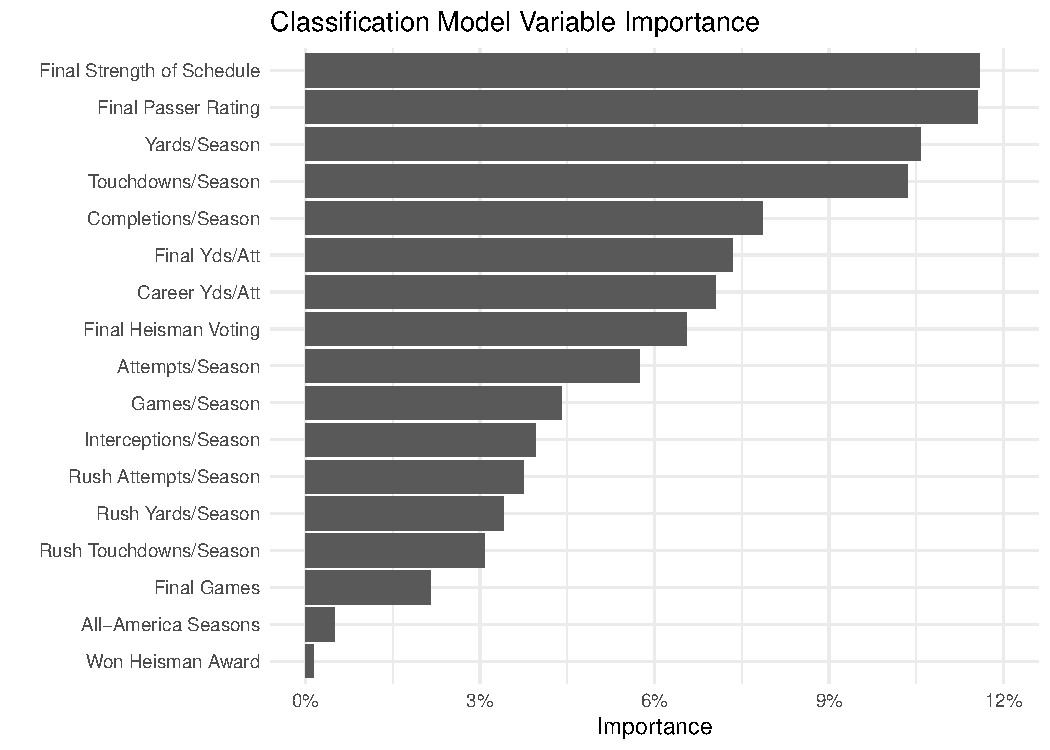
\includegraphics[width=0.49\linewidth]{cls_variable_importance.pdf}
    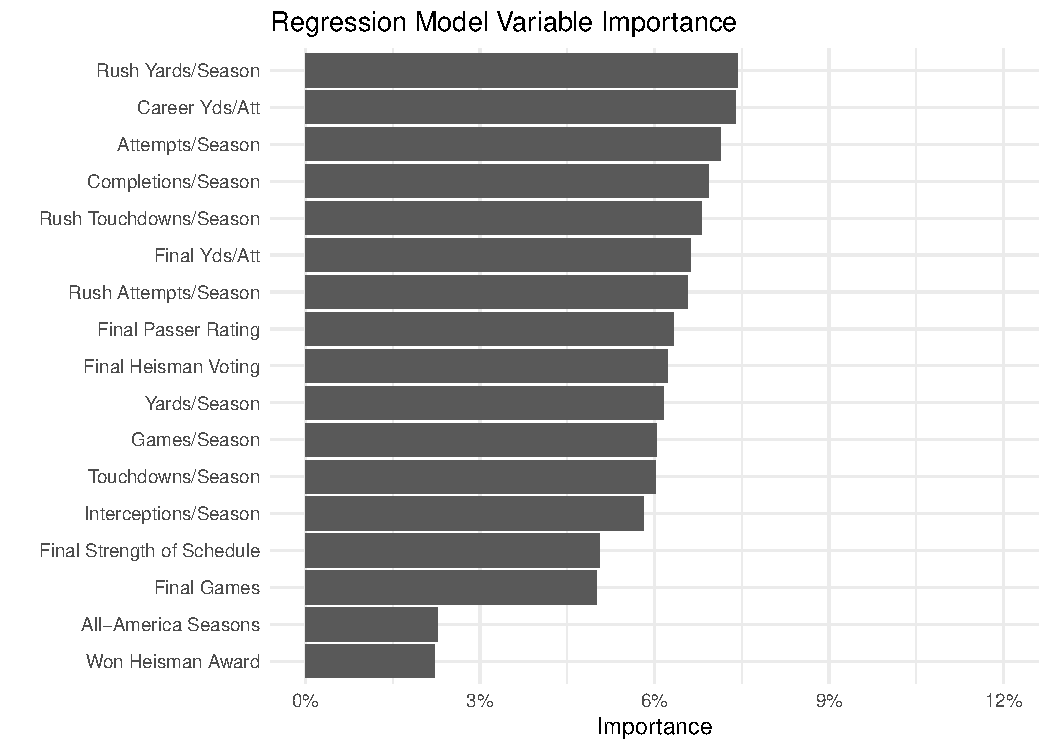
\includegraphics[width=0.49\linewidth]{rgr_variable_importance.pdf}
    \caption{
      \it Feature importance for first-stage (classification) and second-stage (regression) random forests. The first-stage model predicts the probability of nonzero \revision{$\text{QBR}_\text{reg}$} in the NFL, and the second-stage model predicts expected NFL \revision{$\text{QBR}_\text{reg}$} conditional on it being nonzero.
    }
    \label{fig:importance}
\end{figure}

\revision{
  While the feature-based interpretation illustrated by Figures \ref{fig:3d-plot} and \ref{fig:importance} provides interesting macro-level insights on the prediction function learned by the random forest, it does not speak the language of scouting. It does not explain how historical prospect outcomes contribute to current prospect predictions. To translate model predictions into the vernacular of scouting, we need the case-based interpretation of the individual player predictions.
}

\revision{
  To illustrate our case-based approach to interpreting random forest predictions, we focus on the 2025 quarterback draft class. Table \ref{tab:top-ten} shows the $\text{QBR}_\text{reg}$ predictions for the top 10 predicted quarterbacks in the 2025 draft. We highlight four players for interpretation. The first two quarterbacks selected, Cam Ward (first overall) and Jaxson Dart (also first round), were predicted to have the second- and fourth-highest $\text{QBR}_\text{reg}$, respectively. The next quarterback selected, Tyler Shough in the second round, was predicted by the model for only 2.6 $\text{QBR}_\text{reg}$. Dillon Gabriel, the player with the highest predicted $\text{QBR}_\text{reg}$, was selected in the third round.
}

\begin{table}
  \centering
  \resizebox{\textwidth}{!}{
    \begin{tabular}{l|cc|c}
Quarterback & P(QBR $>$ 0) & E[QBR $|$ QBR $>$ 0] & Predicted QBR \\
% latex table generated in R 4.5.0 by xtable 1.8-8 package
% Wed May 20 15:03:36 2026
  \hline
Cameron Ward & 88\% & 38.2 & 33.8 \\ 
  Dillon Gabriel & 87\% & 38.4 & 33.5 \\ 
  Shedeur Sanders & 82\% & 35.1 & 28.9 \\ 
  Jaxson Dart & 64\% & 37.0 & 23.5 \\ 
  Quinn Ewers & 63\% & 33.5 & 21.1 \\ 
  Kurtis Rourke & 69\% & 30.5 & 21.0 \\ 
  Will Howard & 57\% & 33.9 & 19.3 \\ 
  Max Brosmer & 48\% & 33.4 & 15.9 \\ 
  Ollie Gordon & 41\% & 38.3 & 15.6 \\ 
  Davis Sherwood & 44\% & 33.2 & 14.6 \\ 
   \hline
Tyler Shough & 12\% & 26.3 & 3.2 \\ 
\end{tabular}

  }
  \caption{\it Top ten \revision{$\text{QBR}_\text{reg}$} predictions for quarterback prospects in the 2025 draft class. Names in bold are included in Figure \ref{fig:prospect-plots}. Shough's prediction is outside the top ten, but the table includes him for comparison because he was the third quarterback selected in the draft, after Ward and Dart.}
  \label{tab:top-ten}
\end{table}

\revision{Figure \ref{fig:prospect-plots} provides a case-based visualization of how the random forest arrived at its predictions for Ward, Dart, Shough, and Gabriel.} Each prospect's prediction was a weighted average of past prospects' outcomes, and the weighted histograms in Figure \ref{fig:prospect-plots} visualize that weighted mean. Ward had the highest concentration of comps between 55 and 65 \revision{$\text{QBR}_\text{reg}$}, which is why his prediction was the highest of these four prospects. On the opposite end of the spectrum, Shough had the highest concentration of training players near zero \revision{$\text{QBR}_\text{reg}$}, explaining why his prediction was by far the lowest of the four prospects.

\begin{figure}
    \centering
    
\includegraphics[width=0.24\linewidth]{prospect_histogram_ward.pdf}
    
\includegraphics[width=0.24\linewidth]{prospect_histogram_dart.pdf} 
    
\includegraphics[width=0.24\linewidth]{prospect_histogram_shough.pdf}
    
\includegraphics[width=0.24\linewidth]{prospect_histogram_gabriel.pdf}\\
    
\includegraphics[width=0.24\linewidth]{prospect_similarity_ward.pdf}
    
\includegraphics[width=0.24\linewidth]{prospect_similarity_dart.pdf}
    
\includegraphics[width=0.24\linewidth]{prospect_similarity_shough.pdf}
    
\includegraphics[width=0.24\linewidth]{prospect_similarity_gabriel.pdf}\\
    \caption{\it Top: Histogram of historical players' \revision{$\text{QBR}_\text{reg}$} weighted by similarity from the second-stage (regression) random forest, with predicted zero-inflation from the first-stage (classification) random forest. The vertical orange line annotates each prospect's predicted \revision{$\text{QBR}_\text{reg}$}, which matches the mean of the weighted distribution. Bottom: Scatter plot showing individual similarity scores (from the second-stage model) and \revision{$\text{QBR}_\text{reg}$} for historical prospects.}
    \label{fig:prospect-plots}
\end{figure}

\revision{
  Shough and Gabriel provide an interesting contrast because Shough's prediction is so much lower than Gabriel's although Shough was selected before Gabriel in the draft. Table \ref{tab:side-by-side-similarity} provides the ten most similar comps to Shough and Gabriel, separately for the first-stage (classification) random forest and the second-stage (regression) random forest. Among Shough's top first-stage comps, only Jim Sorgi played in the NFL (156 career pass attempts, zero games started). By contrast, all ten of Gabriel's top first-stage comps played and started games in the NFL. Six of Gabriel's top second-stage comps were selected for the Pro Bowl in their careers, compared with none of Shough's top second-stage comps. The similarity scores show that no single comp carries more than 5\% of the weight in the predictions for Shough and Gabriel, meaning that the prediction weight is spread out over many comps.
}

\begin{table}
  \resizebox{\textwidth}{!}{
    \begin{tabular}{lr|lr|lr|lr}
\multicolumn{4}{c|}{Tyler Shough} & \multicolumn{4}{c}{Dillon Gabriel}\\
\multicolumn{2}{c}{Stage 1 (Classification)} & \multicolumn{2}{c|}{Stage 2 (Regression)} & \multicolumn{2}{c}{Stage 1 (Classification)} & \multicolumn{2}{c}{Stage 2 (Regression)}\\
Comp & Score & Comp & Score & Comp & Score & Comp & Score \\
% latex table generated in R 4.5.0 by xtable 1.8-8 package
% Thu May 21 17:03:06 2026
  \hline
Jim Sorgi & 1.6\% & Nathan Peterman & 4.6\% & Mason Rudolph & 2.9\% & Kenny Pickett & 2.3\% \\ 
  Taylor Cornelius & 1.5\% & Mike Kafka & 4.2\% & Dwayne Haskins & 2.7\% & Andrew Luck & 2.2\% \\ 
  Nick Florence & 1.3\% & Greg McElroy & 3.6\% & Andrew Luck & 2.6\% & Trevor Lawrence & 2.1\% \\ 
  Dylan Thompson & 1.2\% & Jim Sorgi & 3.4\% & Trevor Lawrence & 2.5\% & Dwayne Haskins & 2.1\% \\ 
  Clint Chelf & 1.1\% & Skylar Thompson & 3.2\% & Case Keenum & 2.3\% & Case Keenum & 2.1\% \\ 
  Brendon Kay & 1.1\% & Malik Willis & 2.8\% & Bryce Young & 2.1\% & Justin Herbert & 2.0\% \\ 
  Mike Bercovici & 1.0\% & Dennis Dixon & 2.7\% & Kenny Pickett & 2.1\% & Mason Rudolph & 2.0\% \\ 
  Kyle McCann & 1.0\% & Brooks Bollinger & 2.6\% & Baker Mayfield & 2.1\% & Desmond Ridder & 1.8\% \\ 
  Matt Scott & 0.9\% & Josh Allen & 2.2\% & Will Grier & 2.0\% & Aaron Rodgers & 1.6\% \\ 
  Nic Shimonek & 0.9\% & Brock Berlin & 2.1\% & Zach Wilson & 1.8\% & Philip Rivers & 1.6\% \\ 
\end{tabular}

  }
  \caption{\it Top ten similarity scores \revision{from the two-stage random forest for Tyler Shough and Dillon Gabriel}. The similarity score is the contribution made by each historical prospect to the weighted average which constitutes the reference prospect's prediction in the random forest model.}
  \label{tab:side-by-side-similarity}
\end{table}

\subsection{Sensitivity Analysis: Effective Sample Size}

Modifying the model's hyperparameters can result in sparser and more concentrated weights. Figure \ref{fig:ESS-vs-hyperparameter-values} is a box plot showing the relationship between the effective sample size and three random forest hyperparameters. The relationships between ESS and each hyperparameter match intuition. As we increase the maximum depth of the trees, ESS decreases because there are fewer observations in each terminal node. Similarly, as the minimum node size increases, ESS increases because there are more observations in each terminal node. Finally, as we allow ourselves to consider more variables at each split in the tree (greater mtry), ESS decreases because we are more likely splitting on the most important variables again and again, resulting in terminal nodes that look more homogeneous. However, this effect is subtle.

\begin{figure}
    \centering
    
\includegraphics[width=0.9\linewidth]{ESS_vs_hyperparameter_values.pdf}
    \caption{
      \it A visualization of the relationship between random forest hyperparameters and effective sample size (ESS) for player comps. Each box plot represents a distribution of the average quarterback's ESS across 25 scenarios corresponding to differing values of the hyperparameters outside each facet. Hyperparameter details are available in Table \ref{tab:hyperparameters}.
    }
    \label{fig:ESS-vs-hyperparameter-values}
\end{figure}

\begin{figure}
    \centering
    
\includegraphics[width=0.7\linewidth]{comp_pct_plot.pdf}
    \caption{
      \it Cumulative percentage of prediction explained by the top $n$ comparable players, for $n$ from 1 to 184. These calculations are based on similarity scores from the second-stage (regression) random forest. The corresponding effective sample sizes for these prospects are 67.4 for Cameron Ward, 101.1 for Jaxson Dart, 60.7 for Tyler Shough\revision{, and 94.3 for Dillon Gabriel.}
    }
    \label{fig:comp-pct-plot}
\end{figure}

The smaller the ESS, the fewer player comps are needed to explain the random forest predictions for prospects. Figure \ref{fig:comp-pct-plot} shows the number of comparable players required to account for a given share of the prediction weight and states the ESS value for each player in the caption. The curve corresponding to an unweighted average would be a straight line through the middle of the graph. The significant bends in the curves show that there are significant differences in similarity between comps for each prospect. However, this highlights that the top ten comps for each prospect in Table \ref{tab:top-ten} do not tell the whole story of the prediction for each prospect. For each prospect, the top ten comps account for at most 32\% weight in the prediction, and 22-37 comps are required to explain 50\% of the weight in the prediction.

\section{Discussion}
\label{sec:discussion}

\revision{
  With the 40$^\text{th}$ overall pick in the second round, the New Orleans Saints sought a quarterback, with both Tyler Shough and Dillon Gabriel still available on the board. Imagining that the Saints were using a draft model like our two-stage random forest, team executives would want to understand why the predictions were so different for these two players. The decision-makers would need to determine how to weigh Shough's low model prediction alongside his strong maturity, work ethic, and athleticism \citep{mcgavic_tyler_2025}. To do so, they would need to understand how the model arrived at its predictions for Shough and Gabriel.

  Pundits compared Shough with four-time Pro Bowler Jared Goff \citep{campbell_2025_2025} and Super Bowl LII MVP Nick Foles \citep{richard_tyler_2025}, but Table \ref{tab:side-by-side-similarity} presents a less optimistic narrative. Based on the public college performance metrics important for predicting success for NFL quarterbacks, Shough looks more like Nathan Peterman and Mike Kafka, who combined for 176 career passing attempts. Based on those same metrics, Gabriel looks more like Pro Bowlers Trevor Lawrence and Andrew Luck. However, similarity scores are low across the board, highlighting the insight that relying on a single player comp is unwise if the goal is prediction accuracy.

  The random forest prediction may not be better than the scouts' predictions, and this is precisely why interpretability is so important. The model explained 29.7\% of variance in the test set. Evaluating quarterback prospects is notoriously difficult, which is why teams often get it wrong, even with higher-quality proprietary data. The low predictability makes interpretability of predictions even more important because executives cannot rely on a single opaque number. The predictions still carry significant signal, and decision-makers need to understand the source of that signal to effectively synthesize it with other sources of information. The similarity scores extracted from the random forest lay bare its predictions in the vernacular of traditional scouting, facilitating that synthesis.
}

\revision{The specific application of predicting NFL QBR for college quarterbacks is limited by the number of quarterback careers available for training and a low signal-to-noise ratio when using public college performance statistics to predict professional career outcomes. Additionally, the use of $\text{QBR}_\text{reg}$ as the outcome variable presents limitations due to zero-inflation and censoring, as we addressed more deeply in the \nameref{sec:data} section.} Future work could seek a stronger measure of quarterback career outcomes and incorporate additional information from the NFL Draft Combine to explain more of the variance in the outcome. Teammate support, such as strength of receiving corps, may explain additional variance.

\revision{However, the idea of extracting similarity scores from random forests to translate the predictions into the language of player comps in professional sports applies more broadly beyond this specific application.} These similarity scores have the nice property that the random forest predictions are the weighted averages of outcomes in the training set, weighted according to these similarity scores. We have published \revision{the} R package treecomp, which allow\revision{s} researchers and practitioners to extract similarity scores from their own random forest models. Future work could extend \revision{this work} to other tree-based regression and classification models, such as gradient boosting.

%\section{Acknowledgments}
%
%The authors thank Kevin Meers for suggestions that led to improvements in the random forest model for predicting NFL quarterback prospect success.

\section{Author contributions}

EM downloaded the data, calculated the similarity scores, and drafted the manuscript. SP provided the research idea, converted EM's code into an R package, and revised the manuscript.


\section{Statements and Declarations}
\subsection{Ethical Considerations}

Not applicable

\subsection{Consent to Participate}

Not applicable

\subsection{Consent for Publication}

Not applicable

\subsection{Declaration of Conflicting Interest}

The authors declared no potential conflicts of interest with respect to the research, authorship, and/or publication of this article.

\subsection{Funding Statement}

The authors received no financial support for the research, authorship, and/or publication of this article.

\subsection{Code and Data Availability}

The data used for this paper are included in the R package treecomp, which is available at \url{https://github.com/REDACTED/treecomp}. The repository also includes code for reproducing the results in this paper.

\bibliographystyle{SageH}
\bibliography{../random-forest-comps}

\end{document}
